\documentclass[12pt,a4paper]{report}
\usepackage[hmargin=3cm,vmargin=3cm]{geometry}
\usepackage{graphicx}
\usepackage{caption}
\usepackage{array}
\usepackage{listings}
\usepackage{color}
\usepackage{hyperref}
\hypersetup{
	colorlinks=true, % make the links colored
	linkcolor=blue, % color TOC links in blue
	urlcolor=cyan, % color URLs in red
	linktoc=all % 'all' will create links for everything in the TOC
}
\graphicspath{{images/}}

\begin{document}

\begin{figure}
\centering

\includegraphics[width = 0.3\textwidth]{iit}
\hspace{1cm}

\includegraphics[width = 0.4\textwidth]{fossee-logo.png}
\end{figure}

\title{\textbf{\textbf{Summer Fellowship Report}}\vspace{4mm} \\\small On \\\vspace{4mm} \textbf{\large Title}\\ \vspace{4mm}\small Submitted by\\  \vspace{4mm}  \large \textbf{Ashutosh Gangwar}\\ \vspace{1mm} B.Tech (Computer Science and Engineering)\\ MIET, Meerut\\ \vspace{4mm} \large \textbf{Mudit Joshi}\\ \vspace{1mm} B.Tech (Computer Science and Engineering)\\ PDPM IIITDM, Jabalpur\\ \vspace{4mm} \small Under the guidance of \\ \vspace{4mm}
	\large \textbf{Prof.Kannan M. Moudgalya} \vspace{1mm}\\ Chemical Engineering Department  \vspace{1mm} \\IIT Bombay
}

\maketitle


\newpage
\title{\textbf{\textbf{\LARGE 
\begin{flushleft}
\textbf{Acknowledgment}
\end{flushleft}
}}}
\begin{flushleft}
	The fellowship opportunity we had with FOSSEE Team was a great chance for learning and professional development. Therefore, we consider ourselves as very lucky as we were provided with an opportunity to be a part of it. We are also grateful for having a chance to meet so many wonderful people and professionals who led me though this internship period.
	
	Bearing in mind previous I am using this opportunity to express my deepest gratitude and special thanks to the MD of [Company name] who in spite of being extraordinarily busy with her/his duties, took time out to hear, guide and keep me on the correct path and allowing me to carry out my project at their esteemed organization and extending during the training.
	
	I express my deepest thanks to [Name Surname], [Position in the Company] for taking part in useful decision \& giving necessary advices and guidance and arranged all facilities to make life easier. I choose this moment to acknowledge his/her contribution gratefully.
	
	It is my radiant sentiment to place on record my best regards, deepest sense of gratitude to Mr./Ms. [Name Surname], [Position in the Company], Mr./Ms. [Name Surname], [Position in the Company], Mr./Ms. [Name Surname], [Position in the Company] and Mr./Ms. [Name Surname], [Position in the Company] for their careful and precious guidance which were extremely valuable for my study both theoretically and practically.
	
	I perceive as this opportunity as a big milestone in my career development. I will strive to use gained skills and knowledge in the best possible way, and I will continue to work on their improvement, in order to attain desired career objectives. Hope to continue cooperation with all of you in the future

\end{flushleft}

\listoffigures
\tableofcontents

\chapter{\textbf{Introduction}}
FOSSEE (Free and Open Source Software in Education) project promotes the use of FOSS tools to improve the quality of education in our country. They aim to reduce dependency on proprietary software in educational institutions. They encourage the use of FOSS tools through various activities to ensure commercial software is replaced by equivalent FOSS tools. They also develop new FOSS tools and upgrade existing tools to meet requirements in academia and research. 
Incorporated to FOSSEE program, this fellowship's main aim is to introduce students to the FOSS in various engineering fields and to become a part of this big community.
\\\\
We were selected for this fellowship on the basic of screen task submitted by us. There we got opportunity to work on some of the major open source electronic simulation softwares and are introduced to the Technology Stack they are build on. These technologies include C/C++ Programming, Python, Wxwidget, WxPython, PyQt4,etc. 
\\\\
At the beginning of the fellowship we formulated several learning goals, which we want to achieve:
\begin{itemize}
	\item To understand the functioning and working conditions of a government organisation
	\item To see what it is like to work in a professional environment
	\item To see if this kind of work is a possibility for our future career
	\item To use our knowledge and skills and to further increase them
	\item To learn about organising of a open source project
	\item To enhance our communication skills
	\item To build a professional and social network
\end{itemize}
This report is a short description of our 48 days fellowship under FOSSEE. This report contains our activities that have contributed to achieve a number of our stated goals. Following is the description of the softwares we worked on and changes we have done in them, concluding with the experience we gained.
\section{KiCad}
\href{http://kicad-pcb.org/}{KiCad} is a free software suite for electronic design automation (EDA). It facilitates the design of schematics for electronic circuits and their conversion to PCB designs. KiCad was originally developed by Jean-Pierre Charras. It features an integrated environment for schematic capture and PCB layout design. Tools exist within the package to create a bill of materials, artwork, Gerber files, and 3D views of the PCB and its components.
\\
The Kicad suit has 5 main parts: 
\begin{itemize}
	\itemsep0em 
	\item KiCad – the project manager.
	\item Eeschema – the schematic capture editor.
	\item Pcbnew – the PCB layout program. It also has a 3D view.
	\item GerbView – the Gerber viewer.
	\item Bitmap2Component – tool to convert images to footprints for PCB artwork.
\end{itemize}

\begin{figure}[h]
	\centering
	
\includegraphics[scale=0.3]{KiCad-Logo}
	\caption{Kicad Logo}
	\vspace{5mm}
	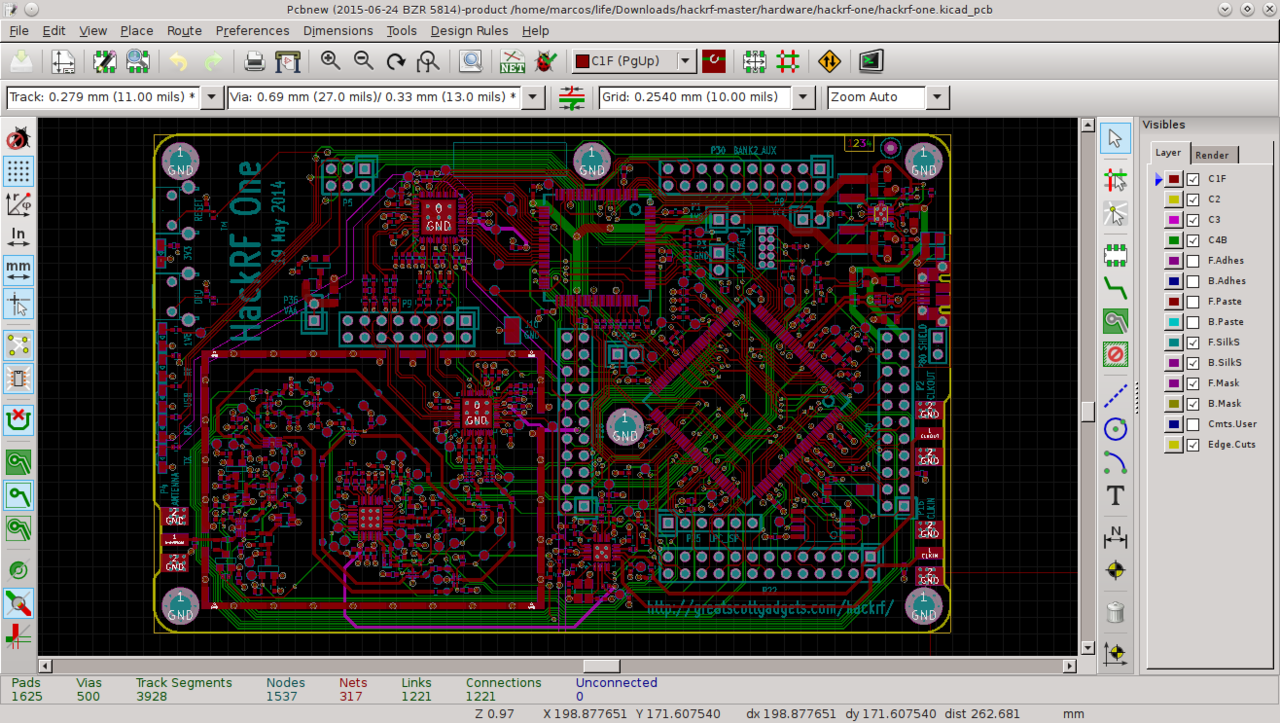
\includegraphics[width=\textwidth]{KiCad}
	\caption{Kicad PcbNew OpenGL}
\end{figure}
\vspace{5mm}

\section{eSim}
\href{https://esim.fossee.in/}{eSim} (previously known as Oscad / FreeEDA) is an open source EDA tool for circuit design, simulation, analysis and PCB design. It is an integrated tool built using open source software such as \href{http://www.kicad-pcb.org}{KiCad} and \href{http://ngspice.sourceforge.net/}{NgSpice}.eSim is released under GPL.
\\
eSim offers similar capabilities and ease of use as any equivalent proprietary software for schematic creation, simulation and PCB design, without having to pay a huge amount of money to procure licenses. Hence it can be an affordable alternative to educational institutions and SMEs. It can serve as an alternative to commercially available/ licensed software tools like OrCAD, Xpedition and HSPICE.
The eSim suit Includes: 
\begin{itemize}
	\itemsep0em 
	\item KiCad  the complete KiCad suit.
	\item KiCadtoNgSpice - Generate Ngspice netlist.
	\item NgSpice Simulation - Simulate Circuit using NgSpice backend
	\item Model Editor
	\item Subcircuit Editor - Design subcircuit fro IC's 
	\item NGHDL - Convert VHDL to Ngspice
	\item Modelica Converter - Convert Modelica files to Schematic
	\item Modelica Optimization
\end{itemize}

\begin{figure}[h]
	\centering
	
\includegraphics[scale=0.2]{eSim-logo}
	\caption{eSim Logo}
	\vspace{5mm}
	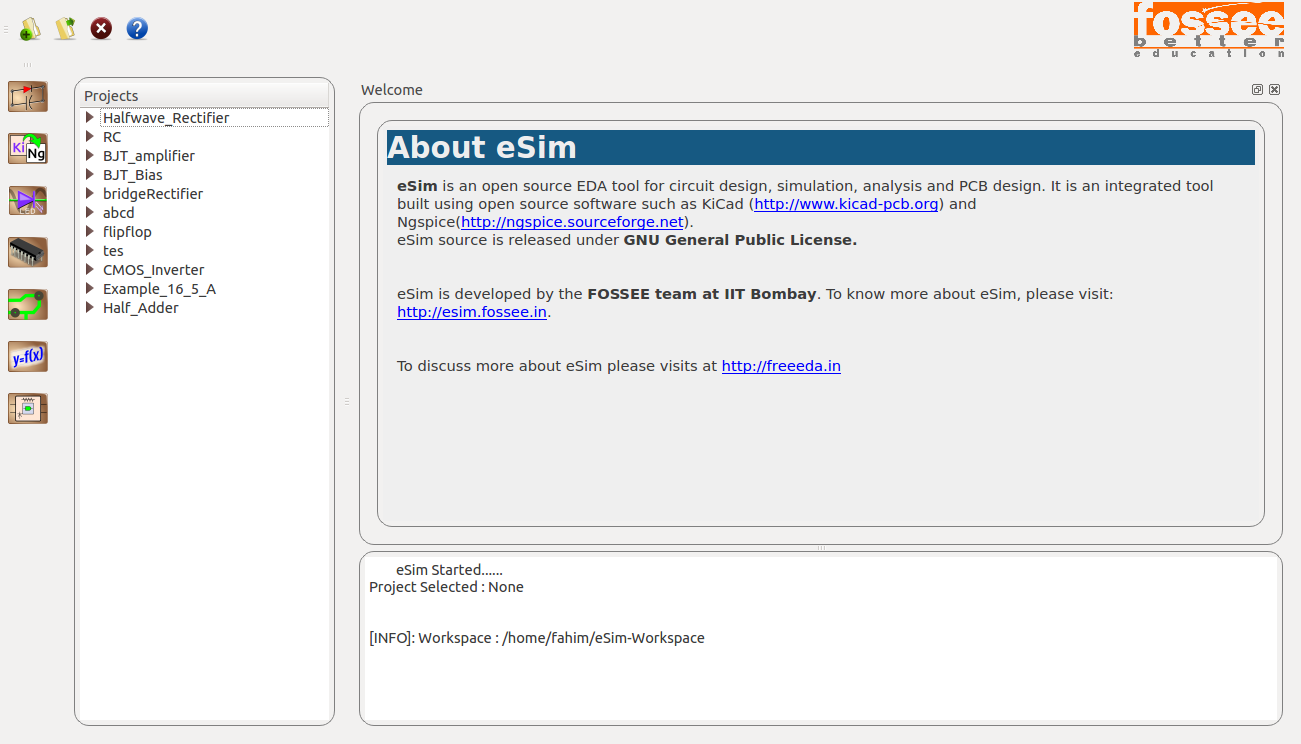
\includegraphics[width=11cm]{eSim}
	\caption{eSim Main Window}
\end{figure}


\section{ngSpice}
Ngspice is a mixed-level/mixed-signal circuit simulator. It is the open-source successor of Spice3f5. A small group of maintainers and the community of motivated users contribute to the ngspice project by providing new features, enhancements and bug fixes.

Ngspice is based on three free-software packages: Spice3f5, Xspice and Cider1b1:
\begin{itemize}
	\itemsep0em
	\item SPICE is the origin of all electronic circuit simulators, its successors are widely used in the electronics community.
	\item Xspice is an extension to Spice3 that provides additional C language code models to support analog behavioral modeling and co-simulation of digital components through a fast event-driven algorithm.
	\item Cider adds a numerical device simulator to ngspice. It couples the circuit-level simulator to the device simulator to provide enhanced simulation accuracy (at the expense of increased simulation time). Critical devices can be described with their technology parameters (numerical models), all others may use the original ngspice compact models.
\end{itemize}

Ngspice is, anyway, more than the simple sum of the packages above, as many people are contributing to the project with their experience, their bug fixes and their improvements giving ngspice additional features and improved robustness.

\begin{figure}[h]
	\centering
	
\includegraphics[scale=0.5]{ngspice-logo}
	\caption{NgSpice Logo}
	\vspace{5mm}
	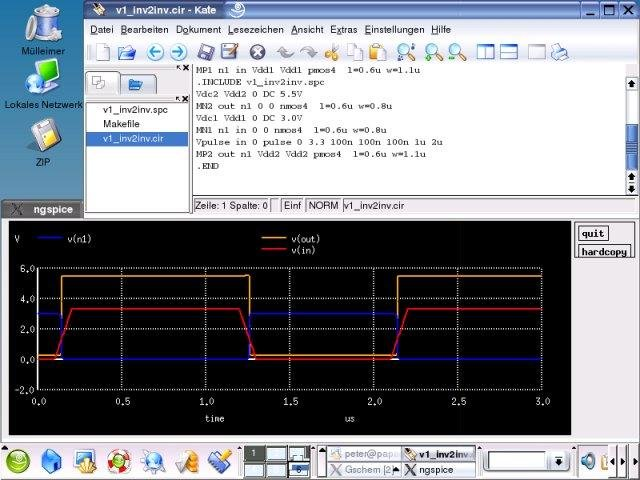
\includegraphics[height=7cm]{ngspice}
	\caption{ngSpice on KDE(Linux)}
\end{figure}


\chapter{\textbf{KiCad Nightly Build (v5)}}
\section{Building KiCad} 
\section{Autoplot PDF when saving projects}
\section{Add hotkey for opening context menu in eeschema}
\section{Ability to open project folder in host operating system}
\section{Inconsistent reference field parsing during editor copy}


\chapter{\textbf{Digital Simulation and Component Parser}}
This Chapter describes about the simulation in ngspice and about the component libraries of Kicad and eSim , similarities and differences between them. Problem description is to find out the reason behind the faliure of ngspice in simulating the digital circuits and some analog circuits in Kicad and to find out if we can use the components of kicad in eSim to increase the eSim library.
\section{Digital Simulation in KiCad}
\section{Parser to increase supported components in eSim}


\chapter{\textbf{eSim}}
\section{Increase External Pins for Sub-Circuits}
\section{Introduced Rename Project Option}
\section{Improve handling of unknown components}
\section{Introduced workspace functionality in eSim}
\section{Minor Bug Fix and improving code usability}

\chapter{\textbf{Standalone Installer for eSim}}

\chapter{\textbf{Conclusion and future work}}

\chapter{\textbf{References}}

\end{document}


